\documentclass{article}

\usepackage{polski}
\usepackage{amsmath, array}
\usepackage{graphicx}
\usepackage{float}
\usepackage{subfig}
\usepackage{multirow}

\title{Laboratorium 1}
\author{\textbf{Łukasz Wala}\\
    \textit{AGH, Wydział Informatyki, Elektroniki i Telekomunikacji} \\
    \textit{Teoria Współbieżności 2022/23}}
\date{Kraków, \today}

\begin{document}
\maketitle

\section{Treść zadania}

\begin{enumerate}
    \item
    Napisać program, który uruchamia 2 wątki, z których jeden zwiększa wartość zmiennej całkowitej o 1, drugi wątek zmniejsza wartość o 1. 
    Zakładając że na początku wartość zmiennej Counter była 0, chcielibyśmy wiedzieć jaka będzie wartość tej zmiennej po wykonaniu 100000 operacji 
    zwiększania i zmniejszania przez obydwa wątki.
    \item
    Na podstawie 100 wykonań programu z p.1, stworzyć histogram końcowych wartości zmiennej Counter.
    \item
    Spróbować wprowadzić mechanizm do programu z p.1, który zagwarantowałby przewidywalną końcową wartość zmiennej Counter. 
\end{enumerate}

\section{Opis rozwiązania}
Pierwszym krokiem rozwiąznia jest napisanie programu:
\begin{verbatim}
class Counter {
    private int _val;
    public Counter(int n) {
        _val = n;
    }
    public void inc() {
        _val++;
    }
    public void dec() {
        _val--;
    }
    public int value() {
        return _val;
    }
}

class IThread extends Thread {
    private Counter counter;

    public IThread(Counter counter) {
        this.counter = counter;
    }

    public void run() {
        for (int i=0; i<10_000; ++i) {
            counter.inc();
        }
    }
}

class DThread extends Thread {
    private Counter counter;

    public DThread(Counter counter) {
        this.counter = counter;
    }

    public void run() {
        for (int i=0; i<10_000; ++i) {
            counter.dec();
        }
    }
}

public class Race {
    public static void main(String[] args) throws InterruptedException {

        Counter cnt = new Counter(0);
        DThread dthread = new DThread(cnt);
        IThread ithread = new IThread(cnt);

        dthread.start();
        ithread.start();
        dthread.join();
        ithread.join();

        System.out.println("state = " + cnt.value());
    }
}
\end{verbatim}

\newpage

Powyższy program został wykonany 100 razy, poniżej znajduje się histogram stworzony na 
podstawie uzyskanych wyników:

\begin{figure}[H]
    \centering
    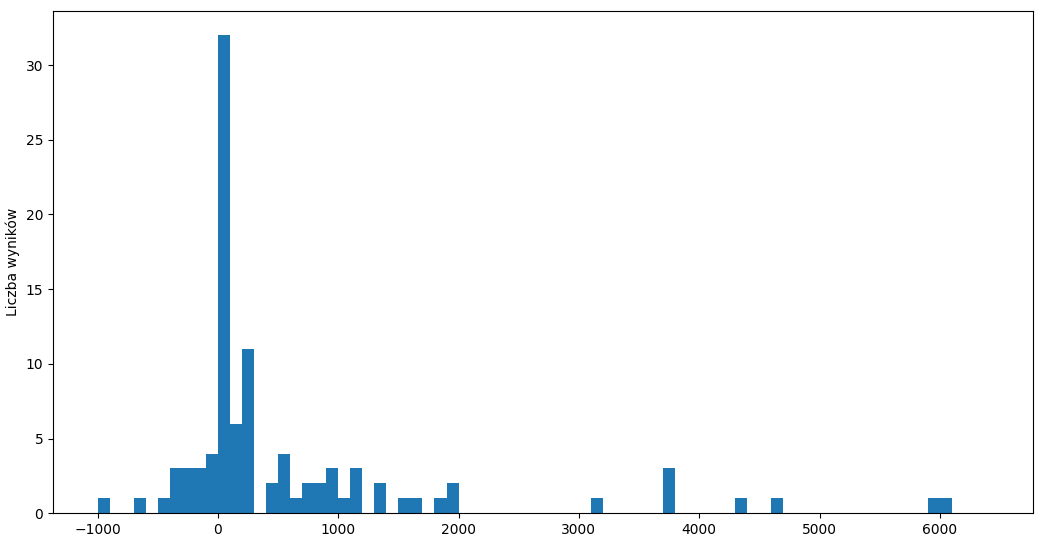
\includegraphics[width=\textwidth]{figure.png}
    \caption{Wyniki dla 100 wykonań programu}
\end{figure}

Możnaby się spodziewać, że dla każdego wykonania wynik będzie wynosił 0, jednak 
inkrementacja licznika nie jest operacją atomiczną (składa się z odczytania zmiennej, 
właściwej inkrementacji i zapisania oraz nie ma gwarancji, że te operacje wykonają się jedna po drugiej).
Przez to operacje dwóch jednocześnie działających wątków mogą się przeplatać i ostateczna wartość 
licznika jest niepoprawna.

Typowym rozwiązaniem tego problemu byłoby użycie narzędzi oferowanych przez system operacyjny zapewniające
atomiczność operacji. W tym przypadku jednak, jako że wątki i tak nie mogą działać prawdziwie równolegle,
bo operują na tym samym liczniku, można dodać warunek, że wątek inkrementujący działa tylko, gdy wartość licznika
jest nieujemna, a wątek dekrementujący tylko wtedy, gdy wartość licznika jest ujemna:

\begin{verbatim}
class IThread extends Thread {
    private Counter counter;

    public IThread(Counter counter) {
        this.counter = counter;
    }

    public void run() {
        for (int i=0; i<10_000; ++i) {
            while (counter.value() > 0)
                ;
            counter.inc();
        }
    }
}

class DThread extends Thread {
    private Counter counter;

    public DThread(Counter counter) {
        this.counter = counter;
    }

    public void run() {
        for (int i=0; i<10_000; ++i) {
            while (counter.value() <= 0)
                ;
            counter.dec();
        }
    }
}
\end{verbatim}

Dzięki temu otrzymywane wyniki są zawsze zgodne z oczekiwaniami. Innym rozwiązaniem byłoby po prostu uruchamianie
wątków synchronicznie (poczekanie przed uruchomieniem drugiego wątku, aż pierwszy skończy pracę), jako że i tak nie
mogą działać prawdziwie równolegle.

\section{Wnioski}

Używanie współdzielonego stanu pomiędzy wieloma wątkami może prowadzić do wielu błędów związanych
z brakiem synchronizacji oraz atomiczność niektórych operacji. Rozwiązaniem może być stosowanie 
systemowych narzędzi do synchronizacji wątków lub unikanie wielowątkowości, kiedy nie jest potrzebna.

\end{document}